\documentclass{beamer}
\mode<presentation> {
%\usetheme{Dresden}
\usetheme{CambridgeUS}
}
\newcommand{\subitem}{\par\qquad}
\usepackage{booktabs}
\usepackage{algorithm}
\usepackage{algorithmic}
\usepackage{tikz}
\usepackage{subfigure}	
\usepackage[round]{natbib}   % omit 'round' option if you prefer square brackets
\DeclareMathOperator*{\argmin}{argmin}
\DeclareMathOperator*{\argmax}{argmax}

\usetikzlibrary{arrows,calc,positioning,decorations.pathreplacing} 
\tikzset{
	>=stealth',
	punkt/.style={
		circle,
		draw=black, thick,
		minimum height=2em,
		inner sep=0pt,
		text centered},
	pil/.style={
		->,
		thick,
		shorten <=2pt,
		shorten >=2pt,},
	cir/.style={
		rectangle,
		rounded corners,
		draw=black, thick,
		minimum width=1.5em,
		text centered},
	arr/.style={
		->,
		thick,
		shorten <=2pt,
		shorten >=2pt,},
	layer/.style={
		draw=black,
		fill=white,
		thick,
		rectangle,
		rounded corners,
		minimum width=1.5em,
		minimum height=12em
	},
	brace/.style={
		thick,
		decoration={
			brace,
			mirror,
			raise=2.5cm
		},
		decorate
	}
}

\newcommand{\drawlayer}[4]{
	\node[layer, draw=#4] (#1) at (#2,#3) {};
	\foreach \x in {-1.75, -1.25, -0.75, -0.25, 0.25, 0.75, 1.25, 1.75} \draw[thick, #4] (#2,\x+#3) circle (0.15);
}
\newcommand\irregularcircle[2]{
	\pgfextra {\pgfmathsetmacro\len{(#1)+rand*(#2)}}
	+(0:\len pt)
	\foreach \a in {10,20,...,350}{
		\pgfextra {\pgfmathsetmacro\len{(#1)+rand*(#2)}}
		-- +(\a:\len pt)
	} -- cycle
}

\newcommand{\independent}{\mbox{${}\perp\mkern-11mu\perp{}$}}
\newcommand{\notindependent}{\mbox{${}\not\!\perp\mkern-11mu\perp{}$}}
\newcommand{\iid}{\overset{\text{iid}}{\sim}}


%%%%%%%%%%%%%%%%%%%%%%%%%%%%%%%%%%%%%%%%%%%%%%%%%%%%%%%%%%%%%%%%%%%%%%%%%%
% PARENTHESES 
%%%%%%%%%%%%%%%%%%%%%%%%%%%%%%%%%%%%%%%%%%%%%%%%%%%%%%%%%%%%%%%%%%%%%%%%%%

\renewcommand{\dot}[2]{\langle {#1},\, {#2} \rangle}
\newcommand{\pa}[1]{\left( #1 \right)}
\newcommand{\pb}[1]{\left\{ #1 \right\}}
\newcommand{\pc}[1]{\left[ #1 \right]}
\newcommand{\pn}[1]{\left\| #1 \right\|}
\newcommand{\ps}[1]{\left| #1 \right|}
\newcommand{\ot}{\leftarrow}
\newcommand{\given}{\, | \,}

%%%%%%%%%%%%%%%%%%%%%%%%%%%%%%%%%%%%%%%%%%%%%%%%%%%%%%%%%%%%%%%%%%%%%%%%%%
% MATHCAL
%%%%%%%%%%%%%%%%%%%%%%%%%%%%%%%%%%%%%%%%%%%%%%%%%%%%%%%%%%%%%%%%%%%%%%%%%%

\newcommand{\D}{\mathcal{D}}
\renewcommand{\P}{\mathcal{P}}
\renewcommand{\Pr}{\mathbb{P}}
\renewcommand{\H}{\mathcal{H}}
\renewcommand{\L}{\mathcal{L}}
\newcommand{\Hk}{{\mathcal{H}_k}}
\newcommand{\F}{\mathcal{F}}
\newcommand{\X}{\mathcal{X}}
\newcommand{\Y}{\mathcal{Y}}
\newcommand{\Z}{\mathcal{Z}}
\newcommand{\N}{\mathcal{N}}
\newcommand{\Ex}{\mathcal{E}}
\newcommand{\Hyp}{\mathcal{H}}
\newcommand{\B}{\mathcal{B}}
\newcommand{\sigm}{\mathrm{sigmoid}}


%%%%%%%%%%%%%%%%%%%%%%%%%%%%%%%%%%%%%%%%%%%%%%%%%%%%%%%%%%%%%%%%%%%%%%%%%%
% MATHBB 
%%%%%%%%%%%%%%%%%%%%%%%%%%%%%%%%%%%%%%%%%%%%%%%%%%%%%%%%%%%%%%%%%%%%%%%%%%

\newcommand{\Pio}{\mathbb{P}}
\newcommand{\R}{\mathbb{R}}
\newcommand{\Rd}{\mathbb{R}^d}
\newcommand{\Rq}{\mathbb{R}^q}
\newcommand{\Rn}{\mathbb{R}^n}
\newcommand{\Rm}{\mathbb{R}^m}
\newcommand{\Rnd}{\mathbb{R}^{n \times d}}
\newcommand{\Rnm}{\mathbb{R}^{n \times m}}
\newcommand{\I}{\mathbb{I}}
\newcommand{\Pa}{\mathrm{Pa}}
\renewcommand{\d}{\mathrm{d}}
\newcommand{\sig}{\mathrm{sign}\circ\!}
\newcommand{\Rp}{R_{\varphi}}
\newcommand{\Rpn}{\hat{R}_{\varphi}}
\newcommand{\Rpnt}{\tilde{R}_{\varphi}}
\newcommand{\f}{f^*}
\newcommand{\fn}{\hat{f}_n}
\newcommand{\fnt}{\tilde{f}_n}
\newcommand{\fntm}{\tilde{f}^m_n}
\newcommand{\Mk}{\M_k}
\newcommand{\muP}{\mu_k(\P)}
\renewcommand{\d}{{\mathrm{d}}}
\newcommand{\Rad}{\mathrm{Rad}}
\newcommand{\M}{\mathscr{M}}
\newcommand{\head}[2]{\multicolumn{1}{>{\centering\arraybackslash}p{#1}}{\textbf{#2}}}
\renewcommand{\do}{do}
\title[Transfer Learning and Causal Inference]{A Meta-Transfer Objective for Learning to Disentangle Causal Mechanisms} 

\author[Behrad Moniri - Mahdiyar Shahbazi]{Behrad Moniri \and Mahdiyar Shahbazi}

\institute[] 
{
Department of Electrical Engineering\\
Sharif University of Technology 
}

\titlegraphic{
\includegraphics[width=2cm]{logo.png}\hspace*{-8.75cm}~%

}
\newcommand{\bigCI}{\mathrel{\text{\scalebox{1.07}{$\perp\mkern-10mu\perp$}}}}
\newtheorem{prop}{Proposition}
\begin{document}

\begin{frame}
\titlepage
\end{frame}

\begin{frame}
\begin{figure}
	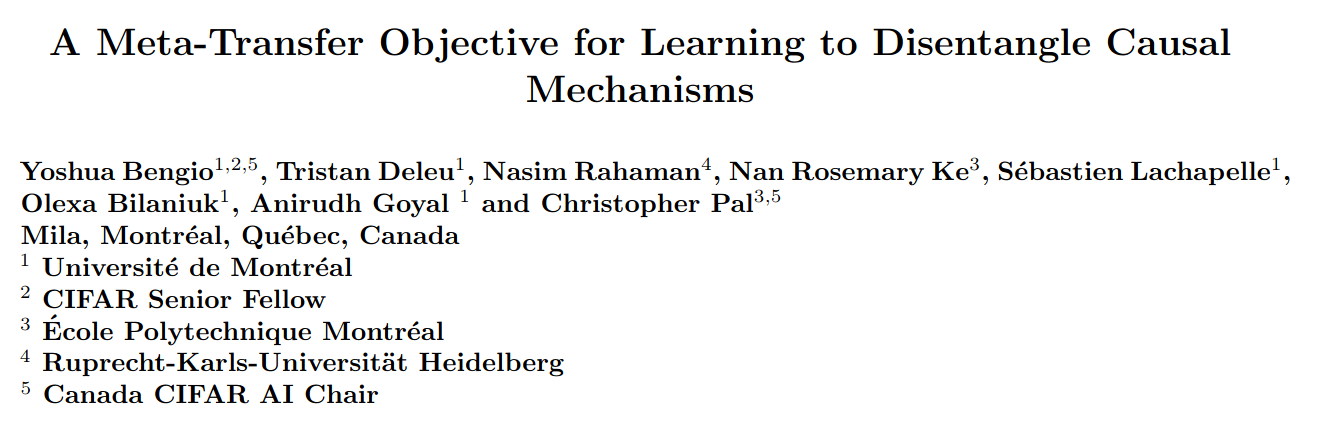
\includegraphics[scale=0.25]{paper.png}
	\\	\textbf{Accepted for ICLR 2020}\\
	\texttt{Code available on Github}
\end{figure}
\end{frame}

\begin{frame}
\frametitle{Introduction}
\begin{block}{Idea 1}
\begin{itemize}
	\item What are the right representations? 
	\item Causal variables explaining the data
\end{itemize}
\end{block}
\pause
\begin{block}{Idea 2}
	\begin{itemize}
		\item How to modularize knowledge for easier re-use \& adaptation, good transfer?
		\item How to disentangle the unobserved explanatory variables?
	\end{itemize}
\end{block}

\end{frame}


\begin{frame}
\frametitle{Hypotheses about how the environment changes}
\Large{\textbf{Main Assumptions:}}
	
\begin{itemize}

	\item Changing one mechanism does not change the others (Peters, Janzig \& Scholkopf 2017)
	
	\item Non-stationarities, changes in distribution, involve few mechanisms (e.g. the result of a single-variable intervention)
\end{itemize}
\end{frame}

\begin{frame}
\frametitle{Claims}
Under the hypothesis of independent mechanisms and small changes across different distributions:

\textbf{smaller sample complexity to recover from a distribution change}\\
E.g. for transfer learning, agent learning, domain adaptation, etc.
\end{frame}

\begin{frame}
\frametitle{Learning a Causal Graph with two Discrete Variables}
If we have the right knowledge representation, then we should get fast adaptation to the transfer distribution when starting from a model that is well trained on the training distribution
\vspace{1cm}

\textbf{Core Idea:  A "Regret" function based on the speed of adaptation.}
\vspace{0.5cm}

However it is clear to us that much more work will be needed to evaluate the proposed approach in a diversity of settings and with different specific parametrizations, training objectives, environments, etc.
\end{frame}

\begin{frame}
Let both $A$ and $B$ be discrete variables each taking $N$ possible values and consider the following two parametrizations

\begin{align*}
\label{eq:bivariate-models}
P_{A\rightarrow B}(A,B)&=P_{A\rightarrow B}(A) P_{A\rightarrow B}(B\mid A) \nonumber \\
P_{B\rightarrow A}(A,B)&=P_{B\rightarrow A}(B) P_{B\rightarrow A}(A \mid B) 
\end{align*}
This amounts to four modules: $P_{A\rightarrow B}(A)$, $P_{A\rightarrow B}(B\mid A)$, $P_{B\rightarrow A}(B)$ and $P_{B\rightarrow A}(A\mid B)$. We will train both models independently.
\vspace{0.3cm}

\textbf{Maximum likelihood estimation of these parameters: normalized relative frequencies.}

$\theta$: parameters of all these models
$$\theta_{A|B}, \theta_{B|A}, \theta_{B}, \theta_{A}$$ 

\end{frame}

\begin{frame}
\frametitle{}
\begin{align*}
\theta_{i} &= P_{A \rightarrow B}(A = i) & \theta_{j|i} &= P_{A \rightarrow B}(B=j\mid A=i)\\
\eta_{j} &=P_{B \rightarrow A}(B=j) & \eta_{i|j}&=P_{B \rightarrow A}(A=i\mid B=j).
\end{align*}

\begin{align*}
\hat{\theta}_i &= n_i / n &\hat{\theta}_{j|i} &= n_{ij} / n_i \nonumber\\
\hat{\eta}_{j} &= n_j / n &\hat{\eta}_{i|j} &= n_{ij} / n_j
\end{align*}

 We can now compute the likelihood for each model:

\begin{align*}
\hat{P}_{A \rightarrow B}(A, B) &= \hat{\theta}_i \hat{\theta}_{j|i} = n_{ij}/n \nonumber\\
\hat{P}_{B \rightarrow A}(A, B) &= \hat{\eta}_j \hat{\eta}_{i|j} = n_{ij}/n
\end{align*}

Which direction can adapt faster? 
Answer: \textbf{The causal direction}
\end{frame}


\begin{frame}
\begin{figure}
\frametitle{Simulation}
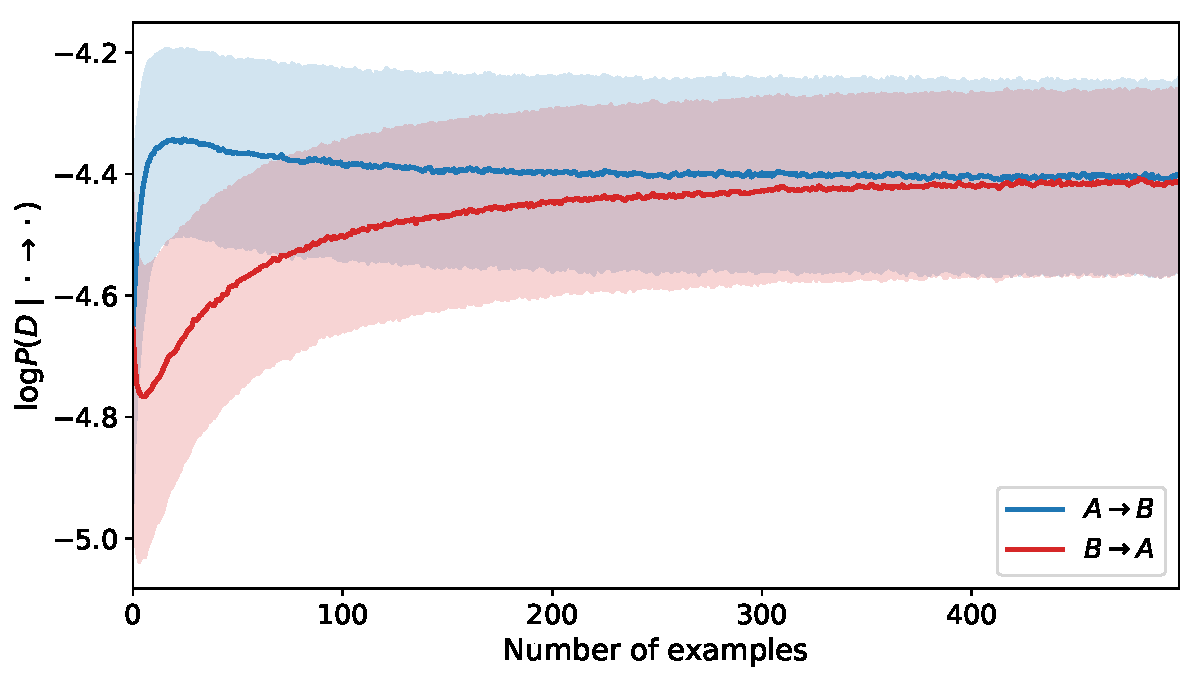
\includegraphics[width=0.9\linewidth]{adaptation-transfer-distribution-discrete-2curves_2.pdf}
\end{figure}
\end{frame}

\begin{frame}
\begin{prop}
	\label{prop:zero-gradient}
	The expected gradient over the transfer distribution of the regret (accumulated negative log-likelihood during the adaptation episode) with respect to the module parameters is zero for the parameters of the modules that (a) were correctly learned in the training phase, and (b) have the correct set of causal parents, corresponding to the ground truth causal graph, if (c) the corresponding ground truth conditional distributions did not change from the training distribution to the transfer distribution. 
\end{prop}
\end{frame}


\begin{frame}
As a consequence, the effective number of parameters that need to be adapted, when one has the correct causal graph structure, is reduced to those of the mechanisms that actually changed from the training to the transfer distribution.
\end{frame}

\begin{frame}
\begin{prop}
	Consider conditional probability modules $P_{\theta_i}(V_i | {\rm pa}(i,V,B_i))$ where $B_{ij}=1$ indicates that $V_j$ is among the parents ${\rm pa}(i,V,B_i)$ of $V_i$ in a directed acyclic causal graph.
	Consider ground truth training distribution $P_1$ and transfer distribution $P_2$ over these variables, and ground truth causal structure $B$. The joint log-likelihood $\mathcal{L}(V)$ for a sample $V$ with respect to the module parameters $\theta$ decomposed into module parameters $\theta_i$ is \mbox{$\mathcal{L}(V)=\sum_i \log P_{\theta_i}(V_i | {\rm pa}(i,V,B_i))$.} 
	If (a) a model has the correct causal structure $B$, and (b) it been trained perfectly on $P_1$, leading to estimated parameters $\theta$, and (c) the ground truth $P_1$ and $P_2$ only differ from each other only for some $P(V_i | {\rm pa}(i,V,B_i))$ for $i \in C$, then $E_{V\sim P_2}[\frac{\partial \mathcal{L}(V)}{\partial \theta_i}]=0$ for $i \notin C$.
\end{prop}
\end{frame}

\begin{frame}

\textbf{The transfer distribution only changed the true $P(A)$ (the cause)}

\begin{itemize}
\frametitle{Bi-Variate Example}
\item
For the correct model only $N-1$ parameters need to be re-estimated.
\item
In the backward model,  all $N(N-1)+(N-1)=N^2-1$ parameters must be re-estimated.
\end{itemize}
\end{frame}



\begin{frame}
\frametitle{More than two parameters}
\begin{itemize}
\item
We won't be able to enumerate all DAGs and pick the best one after observing episodes of adaptation.
\item 
We can
parameterize our belief about an exponentially large set of hypotheses by keeping track of the probability for
each directed edge of the graph to be present
\end{itemize}
\end{frame}

\begin{frame}
\frametitle{Formulization}
\begin{itemize}
\item Modeling edges
\begin{equation*}
B_{ij} \sim {\rm Bernoulli}(p_{ij}), \nonumber \;\;
P(B) = \prod_{ij} P(B_{ij}).
\end{equation*}

\item
The parents of $V_i$, given $B$, as the set of $V_j$'s such that $B_{ij}=1$:
\begin{equation*}
{\rm pa}(i,V,B_i) = \{ V_j \mid B_{ij}=1, \; j\neq i\}
\end{equation*}
\item
The Structural Causal Model:
\begin{equation*}
V_i = f_i(\theta_i, B_i, V, N_i)
\end{equation*}
\begin{itemize}
\item
$N_i$ is an independent noise source to generate $V_i$ 
\item
$f_i$ parametrizes the generator  (active if $B_{ij}=1$)
\end{itemize}
\end{itemize}
\end{frame}

\begin{frame}
\begin{itemize}
	\item
	The conditional likelihood $P_{B_i}(V_i=v_{ti}\mid {\rm pa}(i,v_t,B_i))$ measures how well
	the model that uses the incoming edges $B_i$ for node $i$ performs for example $v_t$.
	
	\begin{equation}
	\mathcal{L}_{B_i} = \prod_t P_{B_i}(V_i=v_{ti}\mid {\rm pa}(i,v_t,B_i)).
	\end{equation}
	\item
	The overall exponentiated regret for the given graph structure $B$ is
	$$\mathcal{L}_B = \prod_i \mathcal{L}_{B_i}$$
	
	\item
	for the generalized multi-variable case
	\begin{align}
	\label{eq:regret}
	\mathcal{R} &= - \log E_B[ \mathcal{L}_B ]
	\end{align}
\end{itemize}
\end{frame}

\begin{frame}
\begin{prop}
	\label{prop:biased}
	The overall regret (Equation~\eqref{eq:regret}) rewrites
	\begin{equation}
	\mathcal{R} = - \sum_i \log \sum_{B_i} P(B_i) \mathcal{L}_{B_i}
	\end{equation}
	and if we are willing to consider multiple samples of $B$ in parallel, a biased but asymptotically unbiased (as the number $K$ of these samples $B^{(k)}$ increases to infinity) estimator of the gradient of the overall regret with respect to meta-parameters can be defined:
	\begin{equation}
	\label{eq:gij}
	g_{ij} = \frac{\sum_k (\sigma(\gamma_{ij})-B_{ij}^{(k)}) \mathcal{L}_{B_i}^{(k)}}{\sum_k \mathcal{L}_{B_i}^{(k)}}
	\end{equation}
	where the $^{(k)}$ index indicates the values obtained for the $k$-th draw of $B$.
\end{prop}
\end{frame}

\begin{frame}
Recall that $\mathcal{L}_B = \prod_i \mathcal{L}_{B_i}$ so we can rewrite the regress loss as follows:
\begin{align*}
\mathcal{R} &= - \log E_B[ \mathcal{L}_B ] \nonumber \\
&= - \log \sum_B P(B) \mathcal{L}_B \nonumber \\
&= - \log \sum_{B_1} \sum_{B_2} \ldots \sum_{B_M} \prod_i P(B_i) \mathcal{L}_{B_i} \nonumber \\
&= - \log \prod_i \left( \sum_{B_i} P(B_i) \mathcal{L}_{B_i} \right) \nonumber \\
&= - \sum_i \log \sum_{B_i} P(B_i) \mathcal{L}_{B_i}
\end{align*}
So the regret gradient on meta-parameters $\gamma_i$ of node $i$ is
\begin{align*}
\frac{\partial \mathcal{R}}{\partial \gamma_i}=& \frac{E_{B_i}[\mathcal{L}_{B_i} \frac{\partial \log P(B_i)}{\partial \gamma_i}]}{E_{B_i}[\mathcal{L}_{B_i}]}
\end{align*}
\end{frame}

\begin{frame}
Note that with the sigmoidal parametrization of $P(B_{ij})$, 
$$\log P(B_{ij})=B_{ij} \log \sigm(\gamma_{ij}) + (1-B_{ij}) \log (1- \sigm(\gamma_{ij}))$$ 
as in the cross-entropy loss. Its gradient can similarly be simplified to
\begin{align}
\frac{\partial \log P(B_{ij})}{\partial \gamma_{ij}} &=
\frac{B_{ij}}{\sigm(\gamma_{ij})} \sigm(\gamma_{ij})(1-\sigm(\gamma_{ij})) \nonumber \\
&\;\;\;\;- \frac{(1-B_{ij})}{(1-\sigm(\gamma_{ij}))}\sigm(\gamma_{ij})(1-\sigm(\gamma_{ij}))) \nonumber \\
&= B_{ij}-\sigm(\gamma_{ij})
\end{align} 
\end{frame}

\begin{frame}
\begin{align*}
\frac{\partial \mathcal{R}}{\partial \gamma_i}=& \frac{E_{B_i}[\mathcal{L}_{B_i} \frac{\partial \log P(B_i)}{\partial \gamma_i}]}{E_{B_i}[\mathcal{L}_{B_i}]}
\end{align*}

A biased but asymptotically unbiased estimator of $\frac{\partial \mathcal{R}}{\partial \gamma_{ij}}$ is thus obtained by sampling $K$ graphs (over which the means below are run):
\begin{align}
g_{ij} = \sum_k (\sigma(\gamma_{ij})-B_{ij}^{(k)}) \frac{\mathcal{L}_{B_i^{(k)}}}{\sum_{k'} \mathcal{L}_{B_i^{(k')}}}
\end{align}

where index $^{(k)}$ indicates the $k$-th draw of $B$
\end{frame}

\begin{frame}
\frametitle{Representation Learning}
\begin{itemize}
\item
So far, we have assumed that the system has unrestricted access to the true underlying causal variables, $A$ and $B$.
\item
This is not always the case!
\begin{equation*}
\begin{bmatrix}
X \\ Y
\end{bmatrix} = R(\theta_{\mathcal D}) 
\begin{bmatrix}
A \\ B
\end{bmatrix}
\end{equation*}
\item
If this is the case, our working assumption -- that the correct causal graph will be sparsely connected, made of independent components, and affected sparsely by distributional shifts -- can not be expected to hold true in general in the space of observed variables.
\end{itemize}
\end{frame}


\begin{frame}
Learn the encoder parameters as well!
\begin{figure}
	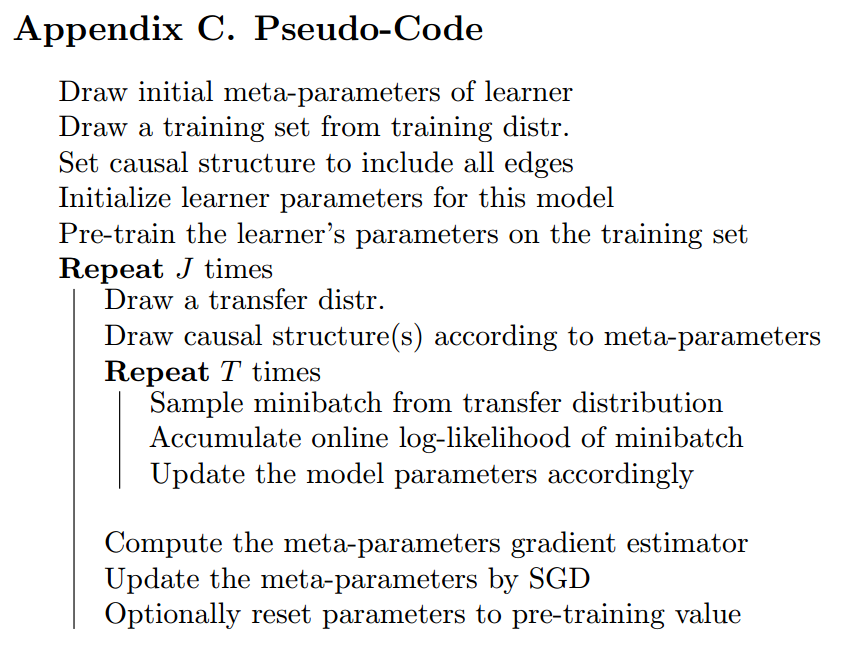
\includegraphics[scale=0.3]{algo.png}
\end{figure}
\end{frame}

\begin{frame}
\frametitle{Future Works!}
This work is only a first step in the direction of optimizing causal structure based on the speed of
adaptation to modified distributions.
\begin{itemize}
	\item This paper has only tested this on artificial data! Can we think of an application?
	\item 
	The representation learning has only been experimentally tested for a very simple rotation matrix!
	
	\item
	Convergence rates for SGD.
	
	\item Biased estimator for the gradient!
	
	\item 
	On the experimental side, many settings other than those studied here should be considered, with different kinds of parametrizations, richer and larger causal graphs, different kinds of optimization procedures, etc.

\end{itemize}
\end{frame}
\end{document}
\begin{frame}
\begin{eqnarray}
\mathcal{R} = -E_B \left[ \sum_{t=1}^T \sum_{i=1}^m \log P_{\theta_{i,t}}(V_i=v_{ti} | {\rm pa}(i,v_t,B_i)) \right]
\end{eqnarray}

\begin{itemize}
	\item
	$\theta_{i,t}$ are the parameters of the $i$-th mechanism (the structural equation for variable $V_i$) at adaptation step $t$ of the transfer episode.
	
	\item
	$v_t$ is the vector of observed values at transfer example $t$.
	\item
	Learning will involve sampling many such episodes, each time with a different $D_2$ sampled from a different transfer distribution (derived as a small change from the training distribution).
\end{itemize}
\end{frame}

